\chapter{Result Analysis}

Initially TORCS-1.3.7 was installed in the system along with all the python modules required to code RL algorithms. Then, a basic python client code is written to communicate with the TORCS server which enables the user establish control over the car. Controlling includes the speed variation, gear selection and steering control. Figures \ref{fig:mainscr}, \ref{fig:tracksel}, \ref{fig:ontrack}, \ref{fig:offtrack} and \ref{fig:offtrack2} are the screenshots obtained during the execution of the program. \\


\begin{figure}[h]
	\centering
	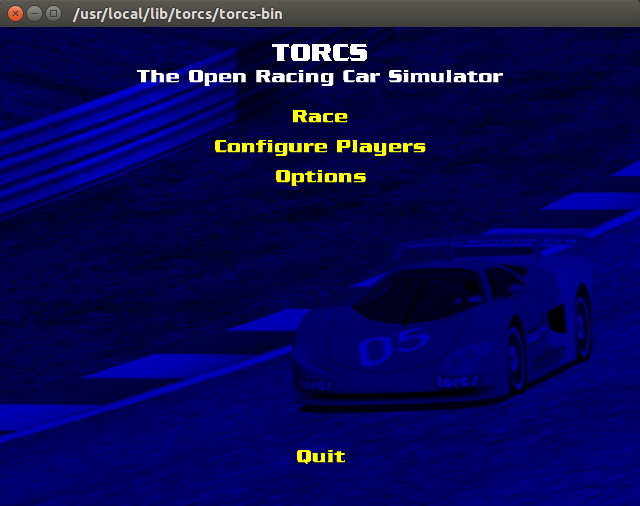
\includegraphics[width=0.6\textwidth]{fig8}
	\caption{TORCS main screen}
	\label{fig:mainscr}
\end{figure}

\pagebreak
\newpage

\begin{figure}[h]
	\centering
	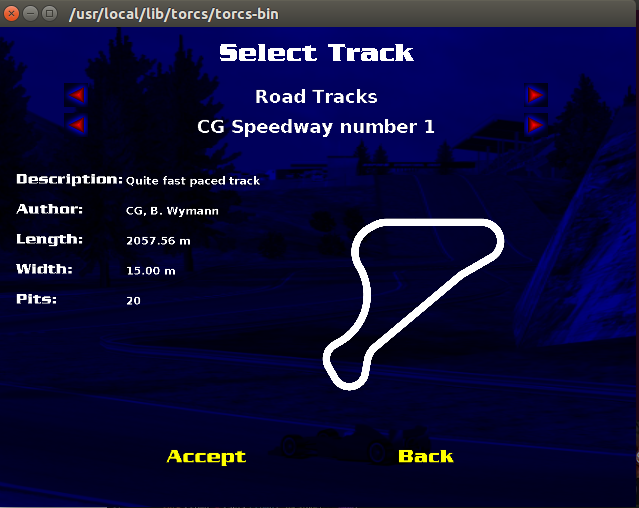
\includegraphics[width=0.6\textwidth]{fig10}
	\caption{Track selection screen}
	\label{fig:tracksel}
\end{figure}


\begin{figure}[h]
	\centering
	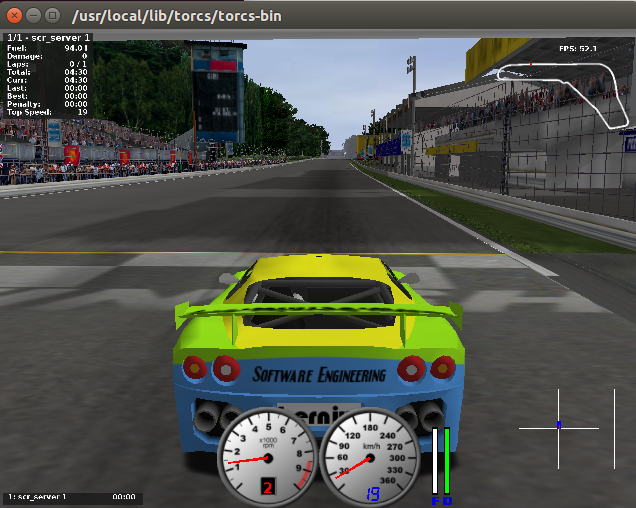
\includegraphics[width=0.6\textwidth]{fig15}
	\caption{Agent driving on the track}
	\label{fig:ontrack}
\end{figure}

\begin{figure}[h]
	\centering
	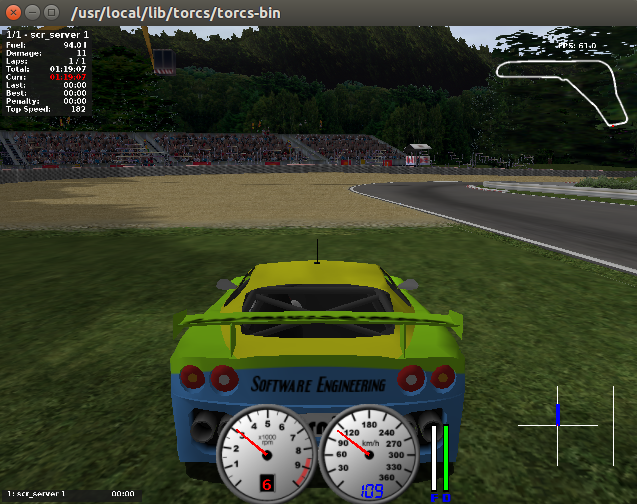
\includegraphics[width=0.6\textwidth]{fig17}
	\caption{Agent goes off-track}
	\label{fig:offtrack}
\end{figure}

\newpage
\begin{figure}[h]
	\centering
	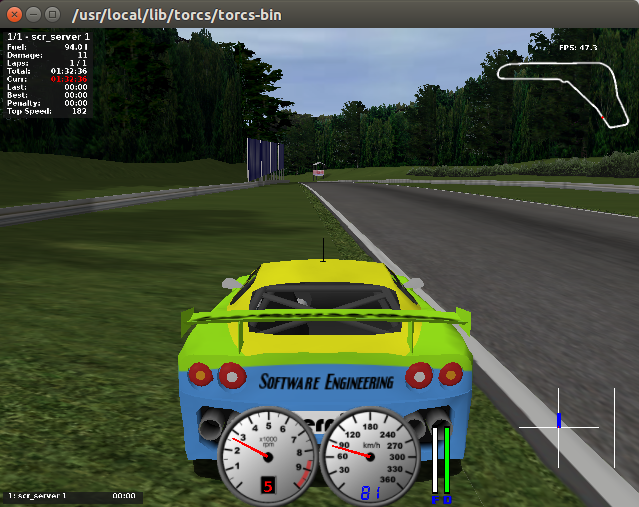
\includegraphics[width=0.6\textwidth]{fig18}
	\caption{Agent slowly getting back on track}
	\label{fig:offtrack2}
\end{figure}

Figure \ref{fig:mainscr} shows the main menu of TORCS simulator .
Figure \ref{fig:tracksel} shows one of the numerous tracks which is available for selection. 
Figure \ref{fig:ontrack} portrays a scenario where the agent is driving on the track. 
Since the agent is not perfectly trained, it sometimes deviates completely off the track as shown in Figure \ref{fig:offtrack}.
However, as soon as it goes out of the track, its rewards begins to diminish. Hence it soon finds its way back to the track as shown in Figure \ref{fig:offtrack2}. 

After the initial training comprising of around 8000 iterations, the agent had learnt to drive on the track but it was not at all moving in a straight line. It was swerving abruptly in its lane. As a solution to this, the learning rate of the actor and critic was altered from 0.001 and 0.002 to 0.0005 and 0.001 respectively to give more time for the agent to learn. This resulted in the agent taking around 14000 iterations to completely re-learn driving from scratch. This is visualized in Figure \ref{fig:res_graph_trg}. Reward obtained in each episode of training is plotted against the episode number. 


\begin{figure}[h]
	\centering
	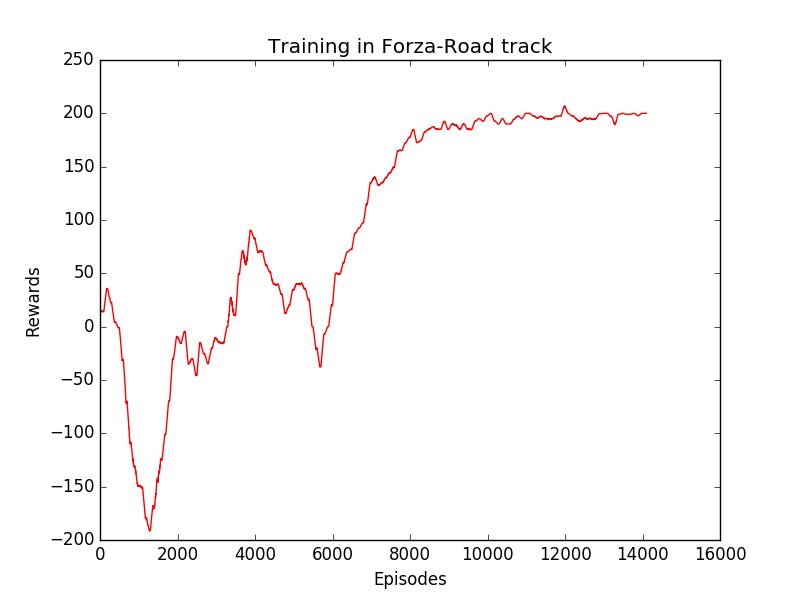
\includegraphics[width=0.7\textwidth]{res_graph_trg}
	\caption{Training of the agent}
	\label{fig:res_graph_trg}
\end{figure}


Figure \ref{fig:res_graph1} shows the variation of rewards with respect to speed(speedX), distance from lane centre(trackPos) and angle between lane and car(theta value). At instances where the speed is less, the rewards follow suit. At times, there are instances where in spite of having sufficiently good speed, the rewards are less. This is due to the fact that the other parameters collectively bring down the rewards as the vehicle may have deviated from the centre of the lane and may have not aligned itself properly with respect to the direction of the lane. In case the rewards are higher than the speed, it shows that the agent has received some extra reward for avoiding some form of probable collision. 

\pagebreak
\newpage

\begin{figure}[h]
	\centering
	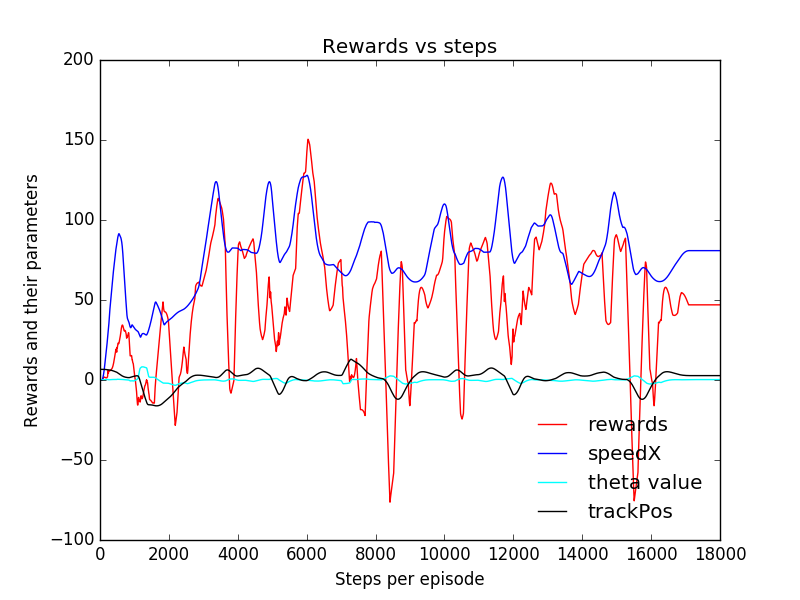
\includegraphics[width=0.7\textwidth]{res_graph1}
	\caption{Rewards vs speed, angle, and position (track 1)}
	\label{fig:res_graph1}
\end{figure}




Figure \ref{fig:res_graph2} further explains the dependency of speed, angle and distance from the centre for rewards. Despite the agent aligning itself properly on the track, it swerved left and right owing to high-speed cornering. 

On careful observation of Figure \ref{fig:res_graph3}, it can be seen that trackPos(distance of the car from the centre of the lane) is very large. In this case, it is larger than +1. This easily translates into the fact that the agent was not driving on the road but beside it. This scenario is created specifically for testing how the rewards would look if the agent is made to not drive on the road. 


Before the agent was trained with an improved learning rate, it was moving in a zig-zag manner in spite of maintaining its lane. Figure \ref{fig:res_graph4} shows how the reward varies if the agent isnt properly trained to drive itself smoothly. 

\pagebreak
\newpage


\begin{figure}[h]
	\centering
	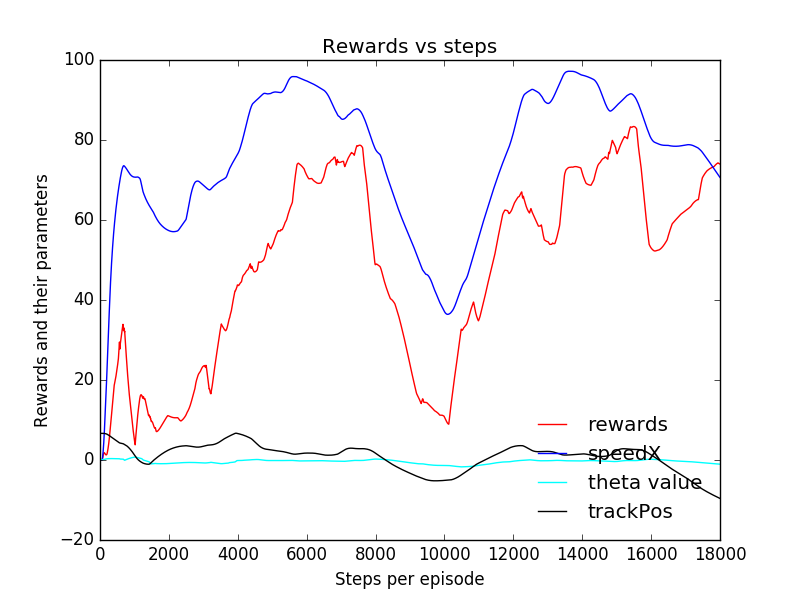
\includegraphics[width=0.7\textwidth]{res_graph2}
	\caption{Rewards vs speed, angle, and position (track 2)}
	\label{fig:res_graph2}
\end{figure}


\begin{figure}[h]
	\centering
	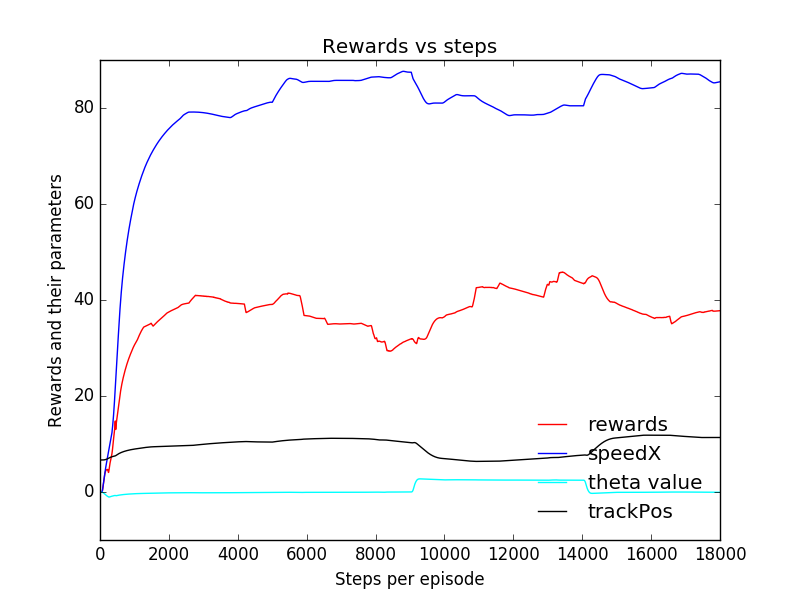
\includegraphics[width=0.7\textwidth]{res_graph3}
	\caption{Rewards vs speed, angle, and position (track 3)}
	\label{fig:res_graph3}
\end{figure}

\pagebreak
\newpage


\begin{figure}[h]
	\centering
	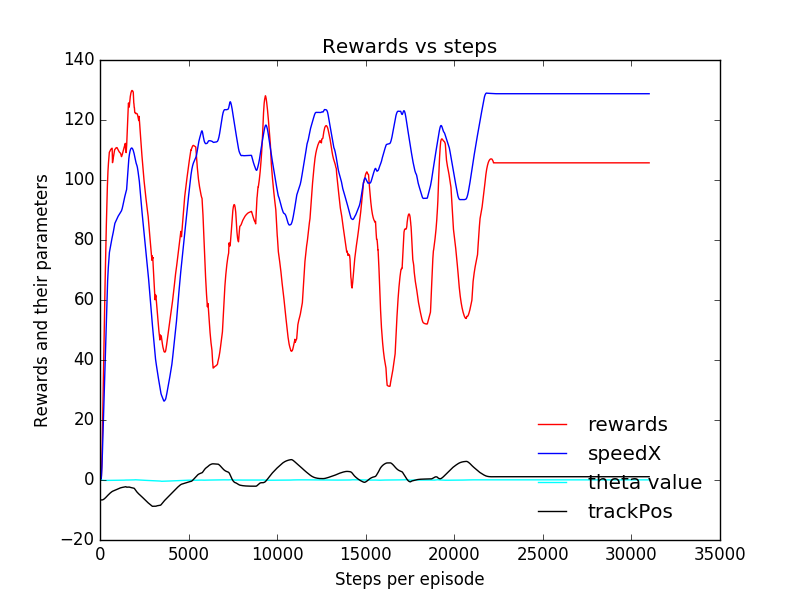
\includegraphics[width=0.7\textwidth]{res_graph4}
	\caption{Rewards vs speed, angle, and position (track 4)}
	\label{fig:res_graph4}
\end{figure}


In all the simulations, the agent successfully managed to drive itself smoothly on the track by constantly interacting with the dynamic environment. It has learnt to detect the twists and turns in the track and applies brakes accordingly. It effeciently detects the obstacles and manages to take precautions or abrupt decisions to avoid collisions. Since all these cannot be depicted here, it is shown in the form of a video available through this link: \href{https://tinyurl.com/jpmrxsyx}{Result Video Link}



%\section{ghf}

%Result analysis
%\begin{itemize}
%\item  Graphical / tabular form/ Screen shots
%\item Explanation for the graphical / tabulated results/ Screen shots
%\item Significance of the result obtained
%\item Any deviations from the expected results and its justification
%\end{itemize}
